\section{Examples of Research Automation Initiatives}
\label{chapter-literature-review}
Since the advent of computers, the history of science can perhaps be described as a history where the automation of science by machines has progressed. The emergence of computational science (computational-X), made possible by high-speed and precise calculations using computers, the rise of data-driven science due to rapid data generation (data-driven science), and the advocacy of e-science are representative examples of this \cite{hey2009fourth}. Gray termed these new scientific practice emerging by the power of computers as new ``paradigms'' of science, borrowing by Kuhn.

Attempts to automate these studies are substitutions of research tasks by machines, and are closely related to the development of machines capable of conducting research. In this chapter, We would like to briefly look back at some of the initiatives related to the automation of research. Then, we will explain how these can be interpreted in terms of the generality and autonomy of research automation. Through this, we hope to provide some insight into where we stand now in terms of realizing artificial intelligence capable of conducting research.
% コンピュータの登場以来の科学の歴史は、計算機による科学の自動化が進んでいった歴史だと言っても良いかもしれません。コンピュータにより高速で性格な計算が可能になったことで登場した計算科学や、高速なデータ生成により生まれたデータ駆動科学などの登場、e-science の提唱などがこれらの例です。これらの研究を自動化する試みは研究タスクの機械による代替ですので、研究ができる機械の開発と密接に関係しています。そこでこの章では、研究の自動化に関するこれまでのイニシアチブのうちのいくつかを簡単に振り返りたいと思います。その後、これらが研究の自動化の汎用性と自律性という観点からどのように解釈しうるかを説明します。これによって、研究ができる人工知能の実現に対して、私たちが今何がどこまでできているのかをざっくり見積もる手助けとなればと思っています。

% 本章では、研究の自動化を目指す試みを幅広く紹介します。特に、これまで同じ論文上やコミュニティ間で論じられることがなかった研究たちも含めて、「研究の自動化を目指す研究群」として統一的に紹介しようと思います。一つ一つの論文を丁寧に紹介することは現実的ではないため、あくまで本論文では各分野や研究の取り組み全体をごく簡単に紹介することに注力します。各分野での研究成果についての詳細な説明については、すでにいくつもの素晴らしいレビュー論文が出版されていますので、そちらをご参照ください。ただし、近年の言語モデルを用いた取り組みについては個別の事例も扱いながら紹介しようと思います。

% 各分野を紹介した後で、汎用的で自律的な人工研究者という観点から、それらを分類する二つの軸を提案します。一つ目が汎用性の軸で、これは各研究の自動化の取り組みが、どれぐらい広い研究領域に対して汎用的なタスクを自動化するものであるかというものです。例えば、科学研究全てで必要となるようなタスクの自動化はある特定の研究課題を自動化するようなものよりも汎用的であると言えます。二つ目が研究過程のどの部分を自動化しているか、という軸です、これは自律性の軸に対応します。例えば、ある研究は仮説生成全体を自動化しているかもしれませんし、別の研究は仮説検証の特定の過程のみを自動化しているかもしれません。全ての研究過程の作業が自動化されている場合、これは自律性が高いと言えます。

% 最後に、研究分野の紹介と軸の提案を踏まえて、研究の自動化に関するパースペクティブ論文・レビュー論文のうちいくつかについて論じます。特に、紹介されている個別の研究よりも、それらの研究がどのようにして既存研究を整理しているか、どのような提案をしているかを見ていきます。これによって、本論文による整理の位置付けを改めて明確にし、次章以降の議論に繋げていきます。

% \section{Examples of Research Automation Initiatives}
We will introduce several examples of initiatives aimed at automating research. The examples introduced here are merely a handful among such initiatives. Furthermore, we have not been able to touch upon specific research outcomes in each initiative. Therefore, this introduction is merely a brief overview and is by no means comprehensive. For more detailed discussions, please refer to survey papers related to each initiative.

% Attempts to automate research began soon after the advent of computers. Until then, humans had developed science by describing experiences (primary science) and by making predictions through the construction of theories (secondary science). With the advent of computers came simulation science (third science), which uses computers to automate complex scientific computations, and data-driven science (fourth science), which automates the discovery of laws from large-scale data \cite{hey2009fourth}. Within the individual academic discipline ``X,'' the third science gave rise to the field of \textit{Computational-X} and the fourth science gave rise to the field of \textit{X-infomatics}, leading to the automation of entire academic disciplines.

\subsection{AI for Science}

\textcolor{red}{TODO: Add literature of applications}

Automation of scientific research with AI, including logical AI, has been an area of interest since the advent of AI \cite{langley1987scientific}. In the early stages of research, researchers created logic AIs that mimics the problem-solving process of researchers \cite{lindsay1993dendral}.

The remarkable performance of deep neural networks has now made almost all scientific fields more or less influenced by AI. The term \textit{AI for Science}, which automates scientific research with machine learning, has appeared due to the remarkable development of machine learning technology since the 2010s. 

AI for Science is a concept that encompasses a very wide range of initiatives. All attempts to solve problems in any process within science using machine learning or to develop the foundational technologies for them can be considered within the scope of AI for Science. Indeed, a vast number of machine learning application studies have been generated in numerous scientific fields \cite{xu2021artificial}, such as AI for Material Science and AI for Medical Science, named few.
\footnote{In this paper, it is not possible to introduce each of these individually, so we will omit the introduction of application studies in each research area of AI here. There are several excellent review papers available, so if you are interested, please refer to those.}
Therefore, it can be said that some of the initiatives we will introduce next are, at least in part, included in the broader concept of AI for Science.

As a general review paper of this fields, Wang et al. have nicely organized existing research on AI for Science by focusing on which phase of
the research process they relate to, whether it’s data collection, hypothesis generation, or hypothesis
verification. \cite{wang2023scientific}. Another detailed review is by Zhang et al., in which they classify existing research based on the temporal and spatial scales of the subjects they address \cite{zhang2023artificial}. Additionally, they emphasize that symmetry is a universally important element across
these different scales and characterize the research from the perspective of symmetry. Xu et al. \cite{xu2021artificial} surveyed the applications of machine learning in eight scientific domains, information science (informatics), mathematics, medical science,
materials science, geoscience, life science, physics, and chemistry.

% Wang et al. \cite{wang2023scientific} have excellently summarized these activities, we will introduce existing automation efforts while borrowing the view of their work. They categorize and organize various initiatives in AI for Science by focusing on which scientific processes they are related to: data handling, hypothesis generation, and simulation and experimentation \cite{wang2023scientific}. This is based on the view that the essence of science lies in the collection, transformation, and understanding of data.

\subsubsection{Incorporating Scientific Knowledge}

The group of studies that incorporate biases to handle scientific data on AI, giving it information about the governing physical rule, is called \textit{physics-informed machine learning} \cite{karniadakis2021physics}. The incorporated biases include the ability to handle partial differential equations (PDE), symmetry, and intuitive physics \cite{hao2022physics}. Karniadakis et al. \cite{karniadakis2021physics} and Hao et al. \cite{hao2022physics} systematically and clearly summarize existing research from the perspective of which elements of machine learning are modulated by which biases and how they are incorporated. % TODO

The ability to handle PDEs gives us the basis for both the simulation of physical models and the discovery of the law from data, which we will discuss later. Studies that aim for better inductive biases and architectures in deep learning by treating symmetry as a first principle are called \textit{geometric deep learning} \cite{bronstein2021geometric}. Given the importance of symmetry in natural sciences, this group of research also plays a significant role in AI for Science. Zhang et al.  organize existing research in AI for Science across different research domains, focusing on symmetry as one of the common foundational pillars \cite{zhang2023artificial}.

In recent years, with the advancement of large-scale neural networks, there have been efforts to inject scientific knowledge to models pre-training with large corpus of scientific texts \cite{taylor2022galactica,beltagy2019scibert}, and with multimodal data \cite{singhal2023towards}.

\subsubsection{Hypothesis Generation}

The methods for generating hypotheses vary significantly depending on the subject, so there exists a wide range of approaches to automate this process. For example, attempts to generate hypotheses from articles or from scientific data are being undertaken in all research fields. 

One long-standing approach to hypothesis generation by AI is the research focused on discovering symbolic equations that describe scientific laws from data (\textit{equation discovery}). Among the earliest pioneering studies in this area, the BACON system by Langley et al. \cite{langley1987scientific}, and subsequent studies based on it, are well-known. In particular, the research on equation discovery that is mainly studied in the machine learning community is known as \textit{symbolic regression}, which originally started from research that used genetic programming approaches to discover symbolic equations.
 Kramer provides a comprehensive overview of the history of equation discovery research, including early studies that did not utilize machine learning \cite{kramer2023automated}. Famous deep learning approaches include AI Feynman \cite{udrescu2020ai,udrescu2020ai2}, which transformed the problem itself into a simple form and discovered the fundamental physical laws selected from Feynman's physics lectures.

% Symbolic regression is a problem of exploring a combinatorial hypothesis space among hypothesis generation \cite{wang2023scientific}. 
% In science, exploration plays a crucial role, as exemplified by the search for hypothesis spaces and experimental conditions mentioned later. Therefore, methodologies for better automated exploration by machines have been sought, using techniques such as active learning. There is a perspective paper of research automation by Kitano \cite{kitano2021nobel} that focuses on the importance of machine-driven exploration of hypothesis spaces. Kitano points out that current hypothesis selection is value-driven, based on human value criteria, and argues that we should aim for hypothesis generation through exhaustive machine-driven exploration that is not dependent on such human value criteria. He points out that some of the Nobel Prize-winning research is actually the result of such exhaustive exploration, emphasizing the importance of this approach.
% \subsubsection{Symbolic Regression / Equation Discovery}
% % \subsubsection{Symbolic Regression} 
% Scientists have constructed models in the form of mathematical equations that explain them from observational data. This has enabled us to go beyond observational data to understand and predict underlying phenomena. That is to say, formulating a mathematical representation that elucidates the phenomenon behind the data is an extremely critical step in science. 

% One attempt to automate this endeavor is \textit{symbolic regression} \cite{makke2022interpretable}, or \textit{equation discovery}. These are attempts to infer from the data a formula that explains it. While classical approaches to symbolic regression have traditionally employed methods such as evolutionary computation, recent years have seen the emergence of strategies utilizing deep neural networks \cite{petersen2019deep,udrescu2020ai,udrescu2020ai2,cranmer2020discovering,kamienny2022end,d2022deep}. Some researchers have proposed the frameworks \cite{landajuela2022unified,keren2023computational} and benchmarks \cite{matsubara2022rethinking} for symbolic regression. You can find a literature review of symbolic regression in \cite{makke2022interpretable}, and that of the early studies in \cite{kramer2023automated}.

\subsubsection{Hypothesis Verification }

Once a hypothesis is formed, it is tested through experimentation. An experiment is the act of generating observational data through a set of predefined procedures. In modern science, simulations are used to generate data that resembles observational data in experimentation. To create better simulations, knowledge of scientific computing is essential. The attempt to automate the generation and analysis of scientific data by combining scientific computing and machine learning is known as \textit{Scientific Machine Learning (SciML)} \cite{baker2019basic}. In physical simulations, numerical solutions to differential equations often come into play, so physics-Informed Machine Learning is also frequently discussed in this context. Experiments and numerical calculations come with uncertainties, so there is a long history of research on quantifying these uncertainties (\textit{uncertainty quantification}). This is also an important topic of study in SciML.

There is also a long history of research applying machine learning to experimental design. In particular, research on the efficient search for experimental conditions using active learning, including Bayesian optimization (\textit{Bayesian experimental design}), or active learning, has been attempted in various application fields.

% 特に科学技術計算と機械学習を組み合わせて科学データの解析を自動化する試みは Scientific Machine Learning (SciML) と呼ばれています。(シミュレーション)

% 機械学習において科学データを扱えるような帰納的バイアスを組み込む研究群は Physics-informed machine learning と呼ばれています。組み込まれるものとしては、直観物理、微分方程式を扱う能力、対称性を抽出する能力などがあります。微分方程式の取り扱いは科学計算がずっと扱ってきたものですので、微分方程式を扱う研究は SciML の文脈で議論されることも多いです。また、対称性は幾何学的構造の保存なので、これらは geometric machine learning の一つとして議論されています。

% データからそのデータの背後の法則を記述するシンボリックな方程式を推定する試みも行われてきた。機械学習を用いてデータから方程式を推論する、symbolic regression がある。方程式を発見するシステムの先駆けとして BACON がある。2000年代には単位による制約から数学的に可能な方程式を同定する研究も行われた。これらは equation discovery という名前で研究されてきました。

\subsection{Automating Physical Experimentation}

\subsubsection{Laboratory Automation}
While AI for Science largely targets the software dimension of scientific research, robotics ventures into automating the hardware aspect, particularly in experimental settings. It has been pointed out that automating experiments in the physical world is crucial yet challenging for the automation of scientific research \cite{coley2020autonomous,zenil2023}. 
 \textit{Laboratory automation}, or \textit{self-driving lab} \cite{abolhasani2023rise}, is a program that seeks to automate empirical research involving scientific experiments that involve interaction with the physical world.

What makes this effort unique compared to other efforts to automate research is that it seeks to automate even manual labor of humans in experimentation by developing robots for experiments to automate the entire process of experimentation. A notable example includes pioneering research in genetics by Ross King, who fully automated the cycle of hypothesis generation, verification, and discovery of new hypotheses with Adam \cite{king2004functional}. Another example is A.I. Cooper, which enabled the use of the same experimental equipment as humans through autonomous robots \cite{burger2020mobile}. 

These examples of initiatives aim to autonomously drive the research cycle, including hypothesis generation, planning and execution of experiments, and generation of hypotheses based on experimental results. Such initiatives are referred to as the closed-loop automation of scientific discovery     \cite{burger2020mobile,king2004functional}. This represents an example of achieving extremely high autonomy in the quest for research automation. Furthermore, there are efforts to develop humanoid robots for experiments, capable of conducting multiple different experiments with a single robot \cite{yachie2017robotic}. This is deemed to be a foundational step towards potentially general research automation.

Many attempts at laboratory automation are specialized for specific experiments. However, efforts are underway to develop humanoid robots capable of conducting experiments \cite{yachie2017robotic}, as well as initiatives to automate the low-level behaviors of robots, towards more general automation.

% A few examples include ``Mahoro'', a general humanoid robot that can conduct various experiments \cite{yachie2017robotic}. The robot could automatically conducted cell culture tasks using \cite{ochiai2021variable}

\subsection{Workflows for Automation}
Workflow is a representation of a process as a sequence of tasks and its dependencies. By designing and running this workflow, the represented process is run automatically.

\subsubsection{Scientific Workflow}
The workflow whose process is a research process, tasks are research tasks that receive and output scientific data is called \textit{scientific workflow} \cite{ludascher2009scientific}. By running scientific workflow systems, research process is automatically executed.  Amidst the flourishing of computational and data-driven sciences with the advancement of computers, these efforts seem to have been conceived to better manage in silico experiments \cite{liew2016scientific}. 

Among such initiatives, just like in the case of laboratory automation, there are efforts that have achieved closed-loop automation, which completely autonomously carries out the cycle of hypothesis generation and verification \cite{gil2017towards}. Gil has presented how machine learning can be incorporated into this scientific workflow \cite{gil2022will}. She also presents a perspective on what kind of AI should be developed in order for it to become a good partner for researchers.

Additionally, there are attempts to design workflows that are reusable beyond individual workflows, in other words, workflows with high generality \cite{hardisty2020canonical}.

% A representative concept of these efforts is \textit{scientific workflow} \cite{ludascher2009scientific}. The work of \cite{gil2022will} expresses an insightful perspective for research automation from the point of this scientific workflow community. She introduced the idea of workflows for automated scientific data analysis and continuous generation, verification, and update of hypotheses. 

\subsubsection{Automated Research Workflow}

In recent years, a more encompassing concept has been proposed, which refers to the entire effort to automate research process tasks using computation, laboratory automation, and tools from AI as an \textit{automated research workflow} \cite{national2022automated}. It might be fair to interpret that this initiative is aiming almost entirely at the automation of research. In the report where this concept was proposed, discussions revolve around how ARW is related to technologies such as the scientific workflow system and ML, how it can address challenges faced by the research industry, and what is needed to promote its adoption \cite{national2022automated}.


\subsection{Automating Formal Science}
While AI for Science largely centers on automating natural sciences, there are also conversations around automating formal sciences like computer science and mathematics.

\subsubsection{Automating Mathematics}
The automation of mathematical proof, \textit{automated theorem proving} (ATP) , has been studied for a long tius. Recently several effort has come up to improve ATP by using machine learning, and especially deep learning. The early seminal work is led by Schulz \cite{schulz2001learning} and Urban \cite{urban2004mptp,urban2008malarea}. The first work applying deep learning to ATP is \cite{irving2016deepmath}. Subsequently, numerous studies have emerged on Automated Theorem Proving (ATP) using deep learning \cite{bansal2019holist}. Recent studies on this topic are well organized by Rabe and Szegedy with a perspective for realizing autonomous mathematician beyond ATP \cite{rabe2021towards}.
% TODO: more organized literature review

There are some studies on the automated theorem discovery not theorem proof \cite{gao2014systematic}. In recent years, attempts have been made to help humans to find mathematical conjectures \cite{davies2021advancing} and
automatically generate mathematical conjectures \cite{raayoni2021generating,mishra2023mathematical}  using machine learning.

Additionally, there has been emerging research on having machines discover better algorithms \cite{mankowitz2023faster,fawzi2022discovering}.

AI for Mathematics: A Cognitive Science Perspective \cite{zhang2023ai}

\subsubsection{Automating Machine Learning}
The attempt to automate various tasks related to machine learning is called \textit{AutoML}. This includes hyperparameter optimization, neural architecture search (NAS), and automation of various pre- and post-processing steps in machine learning. The following website \cite{automlorg} provides a very active overview of AutoML. For literature review, the book \cite{hutter2019automated} explained well about the AutoML by 2019, the paper \cite{bischl2023hyperparameter} and \cite{lindauer2020best,white2023neural} summarizes comprehensively the current state of hyperparameter selection and NAS, respectively. Recently, research has emerged that allows machine learning tasks to be executed with text-based instructions alone \cite{vijay2023prompt}.

Additionally, there is an initiative called MLOps (Machine Learning Operations) that aims to to streamline and automate operations related to machine learning primarily in the business context. This includes automating tasks such as model deployment and continuous training, as well as experiment management. MLOps have tried to automate the laborous tasks that need to be automated to aim for the full automation, such as experiment management, versioning, and deployment. The paper \cite{kreuzberger2023machine} is a good scientific review paper on MLOps.

\cite{zheng2023can}

\subsection{Automating Social Science}

The remarkable performance of the GPT series has led to attempts to automate social science research using these models \cite{bail2023can,ziems2023can,park2023generative,horton2023large}. Wang et al. have explained in detail the studies of large language model applications in social science \cite{wang2023survey}.

\subsection{Scholarly Document Processing}
Most human activities, including research, can be understood as a process of information retrieval from external sources, human processing of the information, and output. In the research context, the information usually is expressed in the form of academic papers. Therefore, automating 
tasks related to research paper is critical. We refer to this kind of automation as \textit{scholarly document processing} \footnote{
This term is taken from the Workshop on Scholarly Document Processing \cite{wssdp}.
}. In this section, not only scholarly document processing automation itself but also initiatives related to it will be briefly introduced.

\subsubsection{Automating Reading, Writing, and Searching}
Scholarly document processing covers automation in areas like paper search, recommendation, information extraction, text generation, and more. Processes related to academic papers can be broadly categorized into: 1. Search: finding papers, 2. Read: extracting information from papers, and 3. Write: generating paper. Therefore, these studies can be categorized into automation of one of these steps.  Some of the these studies are briefly introduced in Appendix \ref{appendix:scholarly-document-processing}. Additionally, there are efforts to develop a database of academic papers to improve the performance of all these tasks, which is also crucial for training large language models \cite{kinney2023semantic}. 

While various studies have existed, the advent of large scale language models has drastically shifted the focus primarily to approaches using these models. With the advent of models like the GPT series \cite{openai2023gpt} and ChatGPT, there's a growing trend of using them for scholarly document processing \cite{alzaabi2023chatgpt}. Some of them have applied it to paper processing \cite{elicit,scispace,van2023chatgpt}, paper search \cite{elicit,scispace}, paper writing \cite{transformer2022can}, abstract generation \cite{gao2023comparing}, literature review generation \cite{aydin2022openai}.

% Processes related to academic papers can be broadly categorized into: 1. Search: finding papers, 2. Read: extracting information from papers, and 3. Write: generating papers. This is because most human activities, including research, can be understood as a process of information retrieval from external sources, human processing of the information, and output. In many cases in research, this information is expressed in the form of papers.

Not limited to papers, but more generally targeting scientific information, Hope et al. formulated research activities as a combination of information retrieval and internal cognitive processing, and presented a perspective on the automation of research tasks by machines \cite{hope2022computational}. They propose a human-focused approach agenda related to research automation, termed ``task-guided scientific knowledge retrieval''. In this concept, AI aids researchers by sifting through vast amounts of research data, selecting information specific to the research tasks. They view research as an interplay between a researcher's internal cognition and the external scientific environment, highlighting the importance of creating algorithms that resonate with the cognitive processes of human researchers and representing and retrieving information that aligns with the inner cognitive world.

\subsubsection{Scientific Language Models/Foundation Models}
In order for us to do scientific research, we must have learned prior knowledge about science. Therefore, research has been done to teach or incorporate such scientific knowledge and assumptions into machine learning models.

One of the most popular approaches today is to create foundational models in science. A foundational model is a pre-trained model that can be adapted to extremely generic downstream tasks. In particular, because language is an extremely general-purpose interface and because language models have developed by leaps and bounds, large-scale language models are now predominantly trained on vast amounts of textual data. In science, scientific large-scale language models have also been developed by training huge amounts of scientific texts, including textbooks and papers \cite{taylor2022galactica}.
% \cite{beltagy2019scibert,singh2022scirepeval,nadkarni2021scientific,cohan2020specter,gupta2022matscibert,taylor2022galactica}.

% \subsubsection{Scientific Language Models}

Whether engaging in reading or writing, the presence of a system that comprehends natural language is indispensable. In recent years, large-scale language models, trained on extensive textual data, have achieved significant success. Concurrently, numerous language models, specifically tailored to scientific documents, have also been proposed \cite{beltagy2019scibert,singh2022scirepeval,nadkarni2021scientific,cohan2020specter,gupta2022matscibert,taylor2022galactica,azerbayev2023llemma}. Furthermore, there are attempts to train foundational models for science using multimodal scientific data \cite{singhal2023towards,takeda2023foundation,nguyen2023climax}.

Indeed, there are studies investigating the scientific knowledge comprehension level of GPT.
\cite{bordt2023chatgpt}.

Applications of GPTs to research \cite{wang2023survey,bran2023chemcrow,jablonka202314}. \textcolor{red}{UPDATE}

\subsubsection{Automating Peer-Review}
One notable example of automating scholarly document processing is the automation of peer review process. Researchers have tried to automate review generation \cite{yuan2022can,yuan2022kid,wang2020reviewrobot}, paper screening \cite{schulz2022future}, research paper assessment \cite{kousha2022artificial}, reviewer assignment \cite{zhao2022reviewer}, and more. As in other fields, recent years have seen research on the automation of peer review using large language models such as GPTs \cite{wexin2023can,liu2023reviewergpt,robertson2023gpt4,hosseini2023fighting}. For traditional research on the automation of peer review, \cite{kousha2022artificial} and \cite{lin2021automated1} have conducted comprehensive literature reviews. In particular, Kousha et al. cover a wide range of topics related to the automation of various aspects of peer review.

% Many studies have tried to automate peer review generation \cite{thelwall2019artificial,schulz2022future,yuan2022can,yuan2022kid,lin2021automated1,lin2021automated2,kumar2022investigations,bharti2022can,uban2021generating,wang2020reviewrobot}. While not generating peer reviews directly, studies focused on automating research paper assessment  can be said to be related to the peer review automation. \cite{kousha2022artificial,li2020multi,huang2018deep}. These studies have proposed the method to assess the quality \cite{thelwall2022predicting,thelwall2022can}, novelty \cite{pelletier2022novelpy,amplayo2019evaluating,shibayama2020measuring}, soundness \cite{cabanac2022decontamination}, and significance \cite{zong2022citation,xia2023review,soni2022predicting,manghi2021new,soni2021follow,van2020schubert,mckeown2016predicting}.

% These investigations concern the automation of processes occurring subsequent to a manuscript's arrival at the hands of reviewers. Conversely, researchers also have investigated the automation before that process, such as determining the appropriate journal for submission \cite{michail2023journal} and assigning the reviewers \cite{zhao2022reviewer}.

% While not centered on automation, certain studies engage in the scientific analysis of the review process \cite{shah2022challenges,verma2021attend,bharti2022confident,bharti2022betterpr,verma2022lack,kennard2022disapere}. These investigations serve to enhance our understanding of the nature of peer review and, in turn, provide valuable insights for the design of more effective automated review methodologies. 

% 数学の定理の証明を自動化する研究は古くから、Automated Theorem Proving (ATP) という名前で研究されています。証明を変換された定理たちをノードにもつ木の探索問題に帰着させるのが基本的なアプローチです。

% より最適な実験条件の決定を自動で行う試みもあります。有名なものはベイズ最適化を用いたベイズ実験計画と呼ばれているものです。

% 学術論文の取得からの情報抽出までを自動化しようという試みも長い研究があります。Scholarly document processing などと呼ばれます。これらはもともと自然言語処理やテキストマイニング、情報検索などのコミュニティで研究されてきました。近年は大規模言語モデルの登場により、多くの課題が解決されました。

% 人間が手作業で行ってきた実験をロボットの力を借りて自動化しようという試みもあります。これらは laboratory automation と呼ばれています。

% 科学における計算の処理とデータの流れを一つのパイプラインとして表現し、それらの処理を自動化しようという研究もあります。これらの研究ではこのようなパイプラインを Scientific Workflow あるいは Automated Research Workflow と呼んでいます。

% 機械学習自体を自動化しようという試みは AutoML として知られています。ハイパーパラメータの探索やアーキテクチャの探索の最適化と自動化などが主に研究されています。また、主にビジネスにおいて機械学習に関連する諸タスクの実行を自動化する取り組みの総体は、MLOps と呼ばれています。

% Peer review を自動化しようという研究も存在します。

% 機械学習の中でも科学研究への応用の文脈でよく言及される分野があります。例えば、active learning, explainable AI, uncertainty quantification, out-of-distribution generalization, exploration、などはこれらの例の一部です。

% 記号的なAIの分野でも早くから研究の自動化の取り組みが行われてきました。例えば、DENDRAL は科学者の思考を自動化したものや、アブダクションなどの推論によって知識発見を自動化しようという試みもある。これらの取り組みは広義には Knowledge Representation and Reasoning という分野の中で盛んに研究が行われてきた。

% While there have been some excellent review articles and perspective papers on previous efforts to automate research, there have not yet been many reviews that deal with these research automation efforts in a shallow or even conservative manner. Therefore, this chapter provides the most comprehensive review possible of research on research automation to date.

% The field related to research automation is vast. While it is not possible to cover all of them, we aim to present as comprehensive an introduction as possible. For this reason, the review of each individual field will be limited to a brief overview. We will introduce survey papers and other literature in those fields, and those who wish to understand more advanced discussions should refer to those references.

% In the following, we will present the past efforts of mankind related to research automation, paying attention to what level of general ``task'' each research automation is oriented toward. This is because efforts to automate research can be interpreted as automating a set of tasks in the research process, or acquiring the ability to do so. Note that the level of generality treated here is naturally not absolute, but is set for convenience. Also, please keep in mind that this classification is for classifying human research activities, so humans are only assumed as the subject of the research. After introducing each effort, we will position these efforts in light of the formulation of the knowledge production process that this paper has dealt with.

% \textcolor{red}{CAUTION: We have not read all of the literature in detail and it may contain errors. We will continue to update this paper, but if you find errors, please contact us or throw us a pull request.}

% \subsection{Reviews and Perspectives}
% So far, we have introduced each of the areas related to research automation. In this section, we will introduce review papers and perspective papers on research related to research automation. Note that the number of review papers on automation in individual research fields is too large to cover them all, so we have only selected review papers that covers wide range of research fields.

% \subsubsection{Survey and Reviews}

% Wang et al. \cite{wang2023scientific} have organized existing research on AI for Science by focusing on which phase of the research process they relate to, whether it's data collection, hypothesis generation, or hypothesis verification.

% Zhang et al. \cite{zhang2023artificial} classify existing research based on the temporal and spatial scales of the subjects they address. Additionally, they emphasize that symmetry is a universally important element across these different scales and characterize the research from the perspective of symmetry.

% Xu et al. \cite{xu2021artificial} surveyed the applications of machine learning in eight scientific domains, information science (informatics), mathematics, medical science,
% materials science, geoscience, life science, physics, and chemistry. 

% The committee of the National Academies of Sciences, Engineering, and Medicine has proposed the concept of ``automated research workflow'' (ARW) as a general term for the movement to automate all aspects of the research process \cite{national2022automated}. They discuss the challenges and potential of ARW while introducing examples of it.
% \subsubsection{Scientific Workflow}
% Gill presents an extremely exciting idea of conducting automated research by turning the entire scientific process into compositional and modular software with the literature review of her and her colleagues' work. \cite{gil2022will}. For example, Gill et al. have created a software of the semantic workflow of scientific data analysis and computation process  \cite{gil2011semantic}. 
% Each step of this workflow modularizes the procedures in research. Not only can these make analysis more efficient, but they also allow for the analysis of the research process itself. Furthermore, common workflows can be identified from multiple workflows, enabling abstraction of cross-domain knowledge about research process. Additionally, Gill and her team have proposed DISK, a systematic framework for hypothesis testing and data analysis. DISK can automatically cycle through a series of processes, including the generation of hypotheses, the determination of data and methods to test them, the acquisition of data from shared repositories, the analysis of that data, and the modification of hypotheses. Furthermore, each hypothesis is associated with information on confidence level and analysis details, which significantly indicates the plausibility of the hypothesis. Additionally, as the hypothesis and its confidence level and analysis are continuously updated and the revision history is retained, it enables the continuous maintenance and update of scientific findings.


% Alien science \cite{kureha2023implications}.

\section{Characterizing Related Works}
In this section, we will organize the existing research from various perspectives. Firstly, we will categorize based on which part of the research process the attempts aim to automate. As we explained in Chapter 2, the research process consists of formulating questions, generating hypotheses, and verifying hypotheses. We will discuss which specific phase each automation effort targets. Following that, we will sort the attempts at research automation from the perspectives of both generality and autonomy.

% \subsubsection{Perspectives}

% Kitano \cite{kitano2021nobel} has proposed as a grand challenge the creation of an AI that autonomously conducts research producing scientific discoveries worthy of a Nobel Prize by 2050. While pointing out that Nobel Prize-caliber research has often resulted from exhaustive exploration, he emphasizes the importance of having AI conduct comprehensive hypothesis searches without relying on subjective human evaluation. In this paper, ideas such as the continuous updating of hypotheses, automation of high-throughput experiments, and the gradual enhancement of autonomy are also presented.
% \subsubsection{Nobel Turing Challenge}
% Kitano also harbors an ambition to automate the entirety of the research process \cite{kitano2021nobel}. This is a thought-provoking paper that is meticulously contemplated. Kitano underscores the ability of AI in automating science to execute exhaustive and thorough exploration as a significant strength. We, as humans, aim to generate hypotheses that yield impactful results (Kitano refers to this as a value-driven approach). However, the importance of research findings is context-dependent, and research that we humans deemed unimportant may become crucial if the presuppositions or the context alter. Kitano proposes to eschew this value-driven approach and implement an alternative, exploration-driven methodology to science, aiming for novel scientific discoveries that were unattainable by human capabilities. Besides, Kitano with many examples and detailed consideration, presents a plethora of stimulating ideas, such as the continuous hypothesis network update, a roadmap to achieve autonomous artificial scientists, and proposition of the Nobel Turing Challenge as a Grand Challenge to substantially advance these endeavors. We highly encourage those interested to delve into this fascinating read.




% Hope et al. \cite{hope2022computational} introduce a human-centric agenda related to research automation, where AI helps humans overcome their cognitive limit by efficiently extracting relevant information from the ever-expanding body of research data, tailored specifically to the tasks researchers are engaged in - a framework they term \textit{task-guided scientific knowledge retrieval}. They start by conceptualizing the act of research as an interaction between a researcher's \textit{inner cognitive world} and the \textit{outer world}, or \textit{scientific ecosystem}. Building on this, they underscore the vital role of representing and retrieving information that aligns with the inner cognitive world of researchers, deftly transforming the cognitive functions used in human research into algorithmic processes.
% \subsubsection{Task-guided Scientific Knowledge Retrieval}
% Hope et al. have written a captivating perspective paper on the automation of research, presenting a fresh and exciting viewpoint \cite{hope2022computational}. They introduce a human-centric idea aimed at efficiently extracting relevant information from the ever-expanding body of research data, tailored specifically to the tasks researchers are engaged in - a framework they term \textit{task-guided scientific knowledge retrieval}. They start by conceptualizing the act of research as an interaction between a researcher's \textit{inner cognitive world} and the \textit{outer world}, or \textit{scientific ecosystem}. Building on this, they underscore the vital role of representing and retrieving information that aligns with the inner cognitive world of researchers, deftly transforming the cognitive functions used in human research into algorithmic processes.

\subsection{Which Processes are Automated?}
In Chapter 2, we proposed the idea that research consists of formulating questions, generating hypotheses, and verifying those hypotheses. In this section, we would like to clarify which of these processes the initiative for research automation aims to automate. As explain before, Wang et al. similarly categorize the efforts of AI for Science based on which parts of the research process are automated \cite{wang2023scientific}. 

% They further categorize hypothesis generation into black-box inference and exploration within both discrete and continuous hypothesis spaces, discussing in detail. Additionally, in validation, they discuss the use cases of AI in experimental design, manipulation, and data generation through simulation. Moreover, they organize applied research on AI, focusing on data handling, such as data generation and representation, instead of question generation.

\subsubsection{Question Construction}

In research automation studies, questions are often given. Research on automatically generating research questions is not as prevalent as automation in other processes. In natural language processing, there is a task of automatically generating questions \cite{pan2019recent,zhang2021review}, but this is done with different motivations than research activities like data augmentation. Automating the construction of questions, or setting the goal behind, is recognized as a challenge that needs to be addressed in the future \cite{coley2020autonomousII,zenil2023,kitano2021nobel}. 

An exception is research that automatically discovers or generates research questions and challenges from the academic literature \cite{lahav2022search,liu2023creative,oppenlaender2023mapping,surita2020can}. For example, Lahav et al. have proposed a methodology for automating the discovery of prevailing challenges within the research community, as well as the emerging hypotheses to address them \cite{lahav2022search}. Oppenlaender and Hämäläinen used GPTs to extract research challenges from HCI papers \cite{oppenlaender2023mapping}. Surita et al. conducted research using techniques of \textit{question generation}, one of the tasks in NLP, to identify the underlying research questions from a paper corpus \cite{surita2020can}. While different from discovering research questions, studies aimed at identifying research trends \cite{krenn2022scientific,krenn2022predicting} are also important in terms of pinpointing significant research directions and can provide insights for research on question discovery.

For question generation, Liu et al. proposed a task to generate research questions for Human Computer Interaction (HCI) and a dataset for that purpose. They evaluated the performance of the baseline model not only in terms of accuracy but also from the perspectives of novelty and surprise \cite{liu2023creative}. Lahat and colleagues had ChatGPT generate research questions related to gastroenterology \cite{lahat2023evaluating}. They found that while it could produce relevant and clear questions, they lacked originality.

There are also attempts to formulate the task of problem generation as a machine learning problem. Zhang has examined, not just in science but more generally, how problem discovery can be formulated, what constitutes a good problem, and how problem discovery can be automatically achieved by machines \cite{zhang2021problem}. % To Challenge?

% Extract research challenges from academic paper with GPT-3.5 \cite{oppenlaender2023mapping}.

% Generating HCI research question with language models \cite{liu2023creative}.

% Research priority identification by ChatGPT \cite{lahat2023evaluating}

% Identifying question behind the academic papers \cite{surita2020can}

% Finding emerging research trends in quantum physics \cite{krenn2022scientific} and AI \cite{krenn2022predicting}.


\subsubsection{Hypothesis Generation}
It is probably fair to say that hypothesis generation is one of the most common processes studied in research automation. Just to name a few, prediction of 3D structures from amino acid sequences, prediction of material structures from desired physical properties, and prediction of newly applicable disease candidates from existing drugs are examples of automated hypothesis generation. In the example given in the previous section, equation discovery, mathematical conjecture generation, knowledge discovery with an abduction algorithm, and hypothesis space exploration are just few examples of this. Wang et al. categorized a group of studies that assist hypothesis generation with AI based on how they utilize AI. They classified these studies into three types: black-box inference by AI, AI-guided exploration of combinatorial hypothesis spaces, and optimization by AI within differentiable hypothesis spaces \cite{wang2023scientific}. 

Many problems related to hypothesis generation are formulated as search problems within the hypothesis space \cite{langley1987scientific}. Indeed, it has been pointed out that typical methods of hypothesis generation in chemical research \cite{coley2020autonomous}, as well as some hypothesis generation methods that have led to Nobel Prize-level research \cite{kitano2021nobel}, are based on such search approaches. Consequently, many studies of automated hypothesis generation propose ways to represent such hypothesis spaces and efficient methods for searching within them. However, as Coley et al point out, currently the hypothesis space to be explored is predefined by humans \cite{coley2020autonomousII}. In that sense, it cannot be said that the machine is truly generating hypotheses from scratch. How to realize open-ended exploration of hypotheses is a challenge in creating an AI capable of hypothesis generation.

% \subsubsection{Hypothesis Generation from Scientific Papers}


Another approach is to generate hypotheses from a group of academic papers \cite{kang2022augmenting,chan2018solvent,wang2023learning,xu2023exploring,yang2023large}. In this method, while a set of papers is specified, the set of hypotheses is not explicitly defined by humans. In this sense, it's a general-purpose methodology. For examples, Kang et al. and Chan et al. have presented studies on automating scientific analogical reasoning for identifying the relationship between problems and their corresponding solutions from a corpus of research papers \cite{kang2022augmenting,chan2018solvent}.

causal inference 

hypothesis-deductive reasoning \cite{vervoort2023criterion}

% For example Portenoy proposed a system that recommend researchers who are pursuing analogous research objectives via divergent approaches \cite{portenoy2022bursting}.el techniques.

% \subsubsection{Others} 

% Some methods have been proposed that don't generate hypotheses directly, but rather assist humans in generating hypotheses from experimental data  \cite{friederich2021scientific}.

 % Hypothesis generation by literature based discovery \cite{wang2023learning}

% Supporting research idea generation with visualization \cite{guo2018topic}

% find research idea (hypothesis) by link prediction and verbalizaation of it \cite{xu2023exploring} <- Hypothesis?

\subsubsection{Hypothesis Verification}
Among the initiatives above, attempts to automate the verification of hypotheses include automated experimental design, laboratory automation, and automated theorem proving. For example, some researchers have tried to automate experimental design for quantum physics \cite{ruiz2022digital} or proposed to design workflow of scientific research as a software \cite{goble2020fair}. Among these, studies attempting to automate physical experiments and workflows in the laboratory are primarily conducted under the domain of laboratory automation, while the rest primarily pertains to the automation of sub-processes of validation that can be completed in the computers.

Wang et al. have categorized groups of studies that utilize AI to assist experiments into areas such as research planning, research guidance, and generating observational data through numerical simulations \cite{wang2023scientific}. Coley et al. discuss in detail the challenges of automating experimental and computational validations, as well as the selection of experiments, while referencing studies on automated verification \cite{coley2020autonomousII}.

% They further categorize hypothesis generation into black-box inference and exploration within both discrete and continuous hypothesis spaces, discussing in detail. Additionally, in validation, they discuss the use cases of AI in experimental design, manipulation, and data generation through simulation. Moreover, they organize applied research on AI, focusing on data handling, such as data generation and representation, instead of question generation.


% Others have proposed machine learning algorithms for formulating and executing experimental designs in a more abstract and simple manner \cite{herrmann2022learning}. 

In recent years, there have been studies attempting to automate the experimentation using language models \cite{boiko2023emergent,charness2023generation,qin2023gpt}.

% Compared to question construction and hypothesis generation, there are few attempts to automate
% hypothesis verification related tasks from the academic literature. Somewhat related is the field of
% scientific claim verification \cite{li2019scientific,wadden2020fact,wadden2022scifact,wadden2022multivers,wang2023using}, which determines the validity of a scientific claim
% through analysis of research paper. This is not the planning or execution of validation, but it is related
% to the automation of validation in the sense that it seeks to understand the validity of scientific claims.
% Since it is an assessment of the validity of a study, the findings of this study may have implications
% for the automation of peer-review

% Most research on research automation automates some tasks in the research process. 

% In contrast, as we introduced above there are attempts to automate the entire research process from start to finish.

% A seminal early works are Adam \cite{king2004functional}, and Eve \cite{williams2015cheaper}. These are closed-loop scientific discovery systems that autonomously execute everything from hypothesis generation to research planning. These systems have logic AI at their foundation. The author of the paper of Adam call these system \textit{robot scientists}, \textit{self-driving labs}, \textit{autonomous discovery}, or \textit{laboratory automation}. Also scientific workflow is also 

% Additionally, the concept of a \textit{scientific workflow}, which represents data and computational processing pipelines in research as software, emerged in the early 2000s. The developments and advances in research related to scientific workflows are consolidated in this literature \cite{barker2008scientific,atkinson2017scientific}. Additionally, these papers \cite{deelman2019role,nouri2021exploring} discusses how machine learning contributes to streamline the each step in the scientific workflow. These are important initiatives in terms of softwareizing the research process \cite{deelman2015pegasus,gil2011semantic}.

\subsection{Generality and Autonomy}

\subsubsection{Autonomy}
As mentioned in the previous section, there are several attempts to automate the entire research process. A seminal early works are Adam \cite{king2004functional}, and Eve \cite{williams2015cheaper}. These are closed-loop scientific discovery systems that autonomously execute everything from hypothesis generation to research planning, based on logic AI and robotics. Furthermore, there is closed-loop automation in some research on automation using scientific workflows \cite{gil2017towards}. These are highly autonomous research automation. Recently, there has also been a movement to create autonomous agents based on language models to tackle scientific problems \cite{wang2023survey}.

However, most of studies on research automation have targeted  only specific tasks within a sub-process of the entire research process. For example, symbolic regression focuses on automating hypothesis generation, while experiment automation pertains to data generation for hypothesis creation and testing.

Furthermore, even in the case of closed-loop research automation,  full automation of all processes of science is yet to be realized \cite{zenil2023,coley2020autonomous,coley2020autonomousII}. One of the biggest issues is that the objectives, problems, and questions of research are given by humans \cite{coley2020autonomousII}. We discussed in Chapter 3 that there are not many studies that have attempted to automate the construction of questions. And while we pointed out in Chapter 2 that automating the construction of questions can lead to an infinite regress from the perspective of autonomy, specifying the high-level goals underlying the questions remains a significant challenge \cite{coley2020autonomousII}. Also, even after the construction of the question, there is the issue that humans are providing machines with a search space that is far more restricted than what humans themselves are given. For example, generating hypotheses from an open-ended hypothesis space has not yet been realized \cite{zenil2023,coley2020autonomousII}, and to put it in extreme terms, while humans might prepare experimental equipment from scratch, machines are given those as a given. 

% To begin with, the realization of a fully autonomous artificial intelligence is still one of the major goals yet to be achieved, not just in research. Therefore, a lot more foundational research will likely be needed to accomplish this.

% Many automation studies primarily target specific tasks within a research process. For example, symbolic regression focuses on automating hypothesis generation, while experiment automation pertains to data generation for hypothesis creation and testing. However, as mentioned earlier, some studies, such as automated research workflows and self-driving labs, aim to automate the entire research process. 

% Coley et al. discuss the advancements in automating scientific discoveries in chemistry \cite{coley2020autonomous}. Their discussion is not limited to automating chemistry but extends to the broader context of automation of science. The paper delves into the insightful topics of automated discovery, including defining scientific discoveries and criteria for assessing their autonomy. In the subsequent paper, Coley et al. organized the existing automation studies based on which processes of scientific workflow are automated \cite{coley2020autonomousII}. In that paper, they point out several challenges for science automation, ranging from dataset handling to physical and computational autonomous validation. 

% Autonomous agent for scientific problem \cite{wang2023survey}

% , and in recent years, there are attempts to automate the entire process using language models.

\subsubsection{Generality}
As we have introduced so far, there are several attempts to automate research through versatile approaches. For example, the automatic generation and discovery of hypotheses \cite{kang2022augmenting,chan2018solvent,wang2023learning,xu2023exploring} or questions \cite{lahat2023evaluating,liu2023creative,oppenlaender2023mapping,surita2020can} from research papers is an approach that can automate research across a wide range of academic fields, from the humanities to natural sciences. Additionally, efforts to create general-purpose robots  \cite{yachie2017robotic}, foundation or generalist models \cite{singhal2023towards,taylor2022galactica}, or to incorporate the inductive bias for understanding physics can be considered initiatives towards general-purpose system.

However, most automation studies target specific challenges in particular research fields. It seems that the goal of creating an AI capable of conducting any research is not receiving much attention. As explained in Chapter 2, in order to create such intelligence, it would be necessary to understand the high level concept of research, question construction, hypothesis formulation, and hypothesis verification, and to be able to execute them appropriately depending on the subject at hand.
% The first and most versatile ability is the ability to perform any task a human being can perform. This includes, for example, the ability to think, to manipulate language, and to act. Second, there are abilities that are required for any research. These include the ability to ask questions, generate hypotheses, and test hypotheses, as explained in Chapter 2. The ability to manipulate the scholarly literature and to search for information are also included in these abilities. This is because research is the activity of producing knowledge from arbitrary inputs, and information retrieval is essential for obtaining inputs, and manipulation of the academic literature is essential for processing and outputting these inputs. So far, this is the capability required for all research.

% Next, there are fields of study that involve some form of quantity in order to do the research. If there are basic quantities involved, whether in the natural or social sciences, then this is the field. These research fields require the ability to manipulate mathematics in some form. In those fields that require the use of empirical methods, which are research methods for generating and analyzing data, you need to be able to use statistics and data analysis.

% And there are abilities that are universally needed within each discipline, such as natural sciences, social sciences, and humanities. For example, in the natural sciences, the ability to perform experiments that interact with the physical world is an essential skill in a very broad range of natural sciences.

% Below that, the generality of tasks and the ability to acquire them gradually narrows down to abilities that are widely needed within each discipline as a whole, such as physics, chemistry, biology, and medicine, and then to abilities needed in even smaller disciplines, such as condensed matter physics, organic chemistry, and molecular biology, and so on.

% Fig. \ref{fig:generality_level} represents the hierarchical structure of generality of tasks we have discussed above. Of course, in actual research, the disciplines are closely related to each other, and such a hierarchical structure is not perfect. What we want to emphasize here is that there are differences in the degree of generality of the technologies to be automated and the capabilities to acquire them, and that each automation effort can be considered distinct in terms of its degree of generality. In the following, we will review the automation efforts of previous studies, focusing on these differences. To emphasize again, this chapter will focus on automation efforts in research related to science in the narrow sense, i.e., the natural sciences.


\begin{figure}[htb]
    \centering
    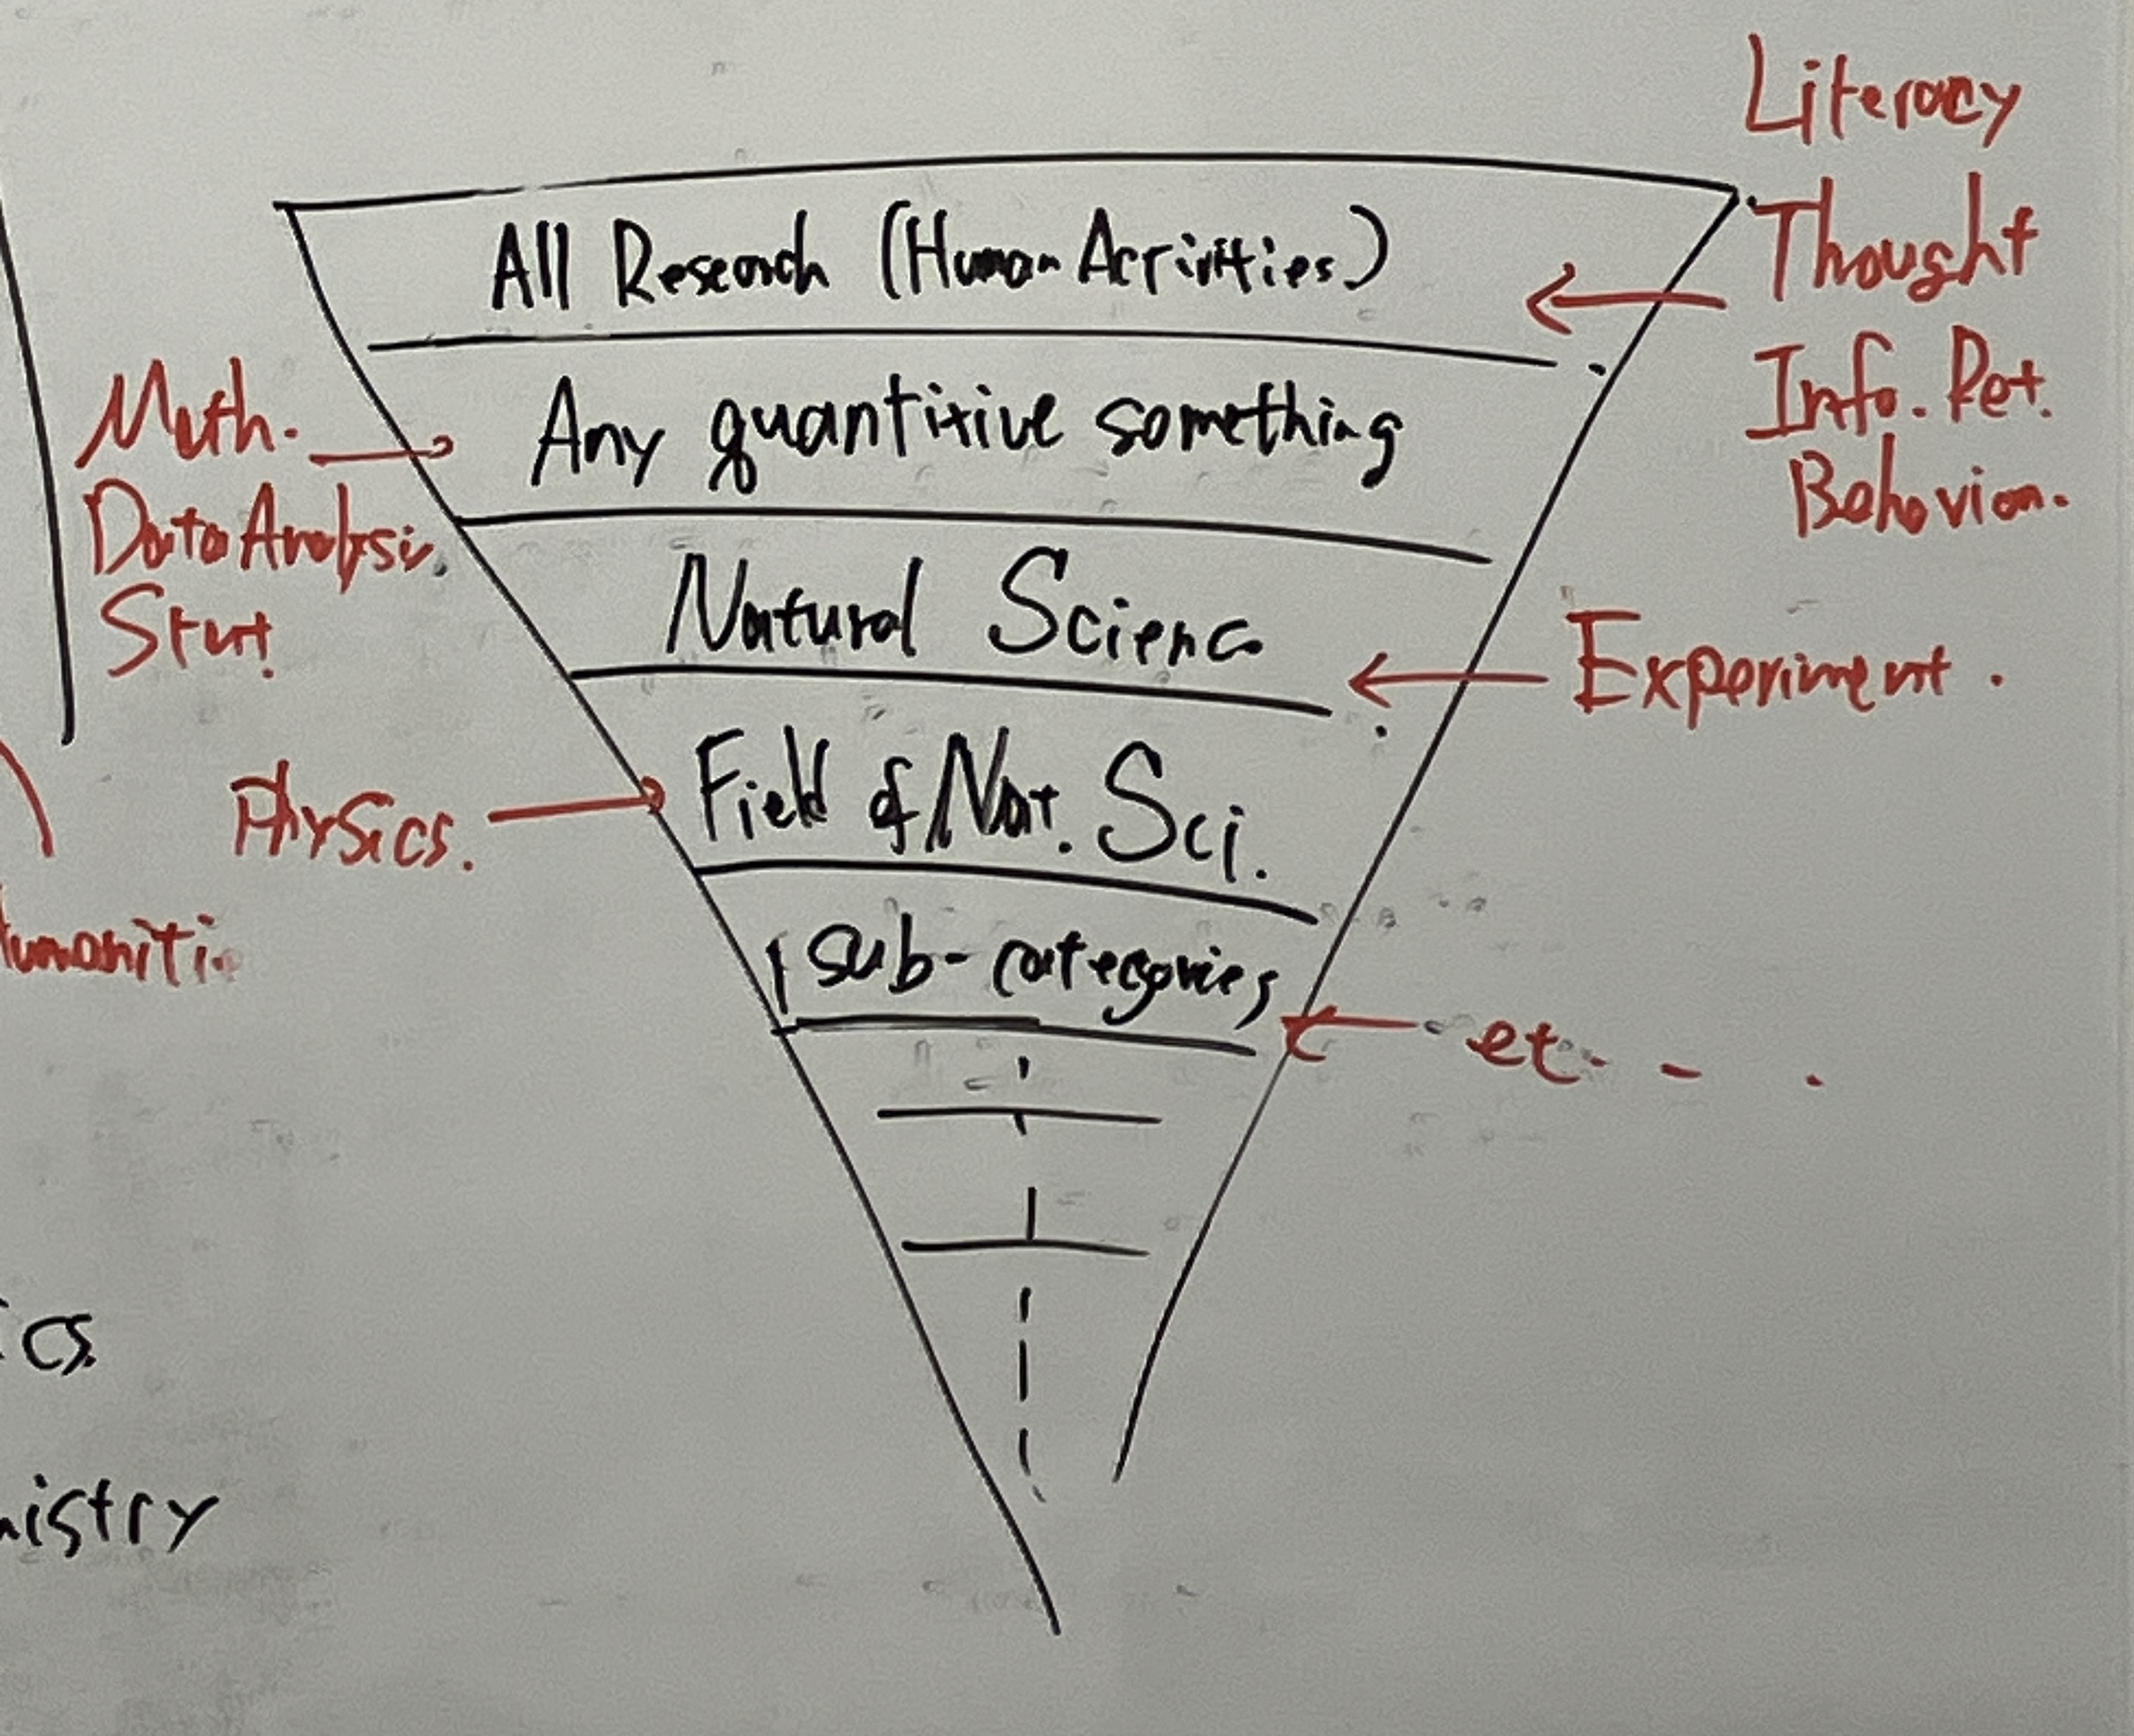
\includegraphics[width=\linewidth]{figs/generality_level.jpg}
    \caption{Caption}
    \label{fig:generality_level}
\end{figure}

% \section{Automation of Tasks for Diverse Field of Research}

% \subsection{Scholarly Document Processing}
% \textit{Scholarly document processing} is a general term for research on automated processing related to scholarly articles and has been studied as part of natural language processing, text mining, and information retrieval.

% \textcolor{red}{TODO: Skip for now. Need reconstruction because many of the issue discussed below are no more issue for research automation. Most of these will moved to Appendix}

% \subsection{Peer Review}
% Many studies have tried to automate peer review generation \cite{thelwall2019artificial,li2019generating,schulz2022future,yuan2022can,yuan2022kid,lin2021automated1,lin2021automated2,kumar2022investigations,bharti2022can,uban2021generating,wang2020reviewrobot}. While not generating peer reviews directly, studies focused on automating research paper assessment  can be said to be related to the peer review automation. \cite{kousha2022artificial,li2020multi,huang2018deep}. These studies have proposed the method to assess the quality \cite{thelwall2022predicting,thelwall2022can}, novelty \cite{pelletier2022novelpy,amplayo2019evaluating,shibayama2020measuring}, soundness \cite{cabanac2022decontamination}, and significance \cite{zong2022citation,xia2023review,soni2022predicting,manghi2021new,soni2021follow,van2020schubert,mckeown2016predicting}.

% These investigations concern the automation of processes occurring subsequent to a manuscript's arrival at the hands of reviewers. Conversely, researchers also have investigated the automation before that process, such as determining the appropriate journal for submission \cite{michail2023journal} and assigning the reviewers \cite{zhao2022reviewer}.

% While not centered on automation, certain studies engage in the scientific analysis of the review process \cite{shah2022challenges,verma2021attend,bharti2022confident,bharti2022betterpr,verma2022lack,kennard2022disapere}. These investigations serve to enhance our understanding of the nature of peer review and, in turn, provide valuable insights for the design of more effective automated review methodologies. 

% \subsection{Cognitive }

% \section{Automation of Tasks for Diverse Fields of Science}
% % There are prerequisite competencies and knowledge required to conduct scientific research. And the question of how to acquire such abilities has been one of the major concerns of AI research for science. Therefore, we will first introduce these research areas. In particular, we will present research on processing scientific literature and understanding scientific knowledge.

% % \subsection{Automated Theorem Proving}



% % \subsection{Understanding Scientific Knowledge}

% % \subsection{AI for Science}

% TODO

% \textcolor{red}{TODO: table for case studies to test the scientific understanding of chatgpt and gpt-4 }

% \subsection{Scientific Machine Learning: Inserting Inductive Bias for Scientific Understanding}
% Another prominent approach to incorporating such scientific knowledge into artificial intelligence is to incorporate inductive biases that help scientific understanding. This area has been studied typically under names such as \textit{scientific machine learning (SciML)} and \textit{physics-informed machine learning}.

% Whereas methods to learn scientific knowledge from the literature are generic methods that learn scientific knowledge through the generic interface of language, in this approach, humans add biases to either the model, the data, or the optimization method that are assumptions of scientific understanding. The constraints that have been studied include the abilities to handle (differential) equations, symmetry, intuitionistic physics, and so on \cite{hao2022physics}. 

% For differential equations, Physics-Informed Neural Networks \cite{raissi2019physics} and Neural Operators \cite{kovachki2021neural} are well known examples of this line of studies. These are methods that enable data-driven simulation of differential equations from data (forward problems) and differential equation discovery (inverse problems). Deep neural networks that can handle symmetry are studied under the name \textit{geometric deep learning} \cite{bronstein2021geometric}. The following survey is comprehensive in this area and should be referred to by those interested \cite{hao2022physics}.

% \subsection{For Empirical Studies}
% Research methods in science can be empirical or non-empirical. Empirical research is research that involves the generation of data, one of the crucial elements in science. Here, we present an effort to automate research on tasks related to scientific data. Machine learning is used in these areas in a variety of ways, including variable selection and model selection, but this section will focus specifically on those areas that have names.

% \subsubsection{Laboratory Automation}
% \textit{Laboratory automation} is a program that seeks to automate empirical research involving scientific experiments that involve interaction with the physical world.

% What makes this effort unique compared to other efforts to automate research is that it seeks to automate the entire process of validation, and it seeks to automate even the manual labor of humans in experimentation. Specifically, they automate human tasks by creating robots that can conduct research. A few examples include ``Mahoro'', a general humanoid robot that can conduct various experiments \cite{yachie2017robotic}. The robot could automatically conducted cell culture tasks using \cite{ochiai2021variable}

% \subsubsection{Bayesian Experimental Design}
% In order to conduct an efficient experiment, it is necessary to properly determine which experimental. \textit{Experimental design}, which involves devising efficient methods for conducting appropriate experiments, has long been studied. \textit{Bayesian experimental design} is an attempt to optimize and automate this experimental design by using Bayesian optimization \cite{chaloner1995bayesian,shahriari2015taking}. Bayesian experimental design has been incorporated from a relatively early stage and has been used in materials science and other fields.


% \subsubsection{Symbolic Regression / Equation Discovery}
% % \subsubsection{Symbolic Regression} 
% Scientists have constructed models in the form of mathematical equations that explain them from observational data. This has enabled us to go beyond observational data to understand and predict underlying phenomena. That is to say, formulating a mathematical representation that elucidates the phenomenon behind the data is an extremely critical step in science. 

% % Modern science is composed of a cycle of observation, hypothesis generation, and hypothesis testing. In many fields, including physics, chemistry, and biology, mathematical models are often constructed as hypotheses from observational data. 

% One attempt to automate this endeavor is \textit{symbolic regression} \cite{makke2022interpretable}, or \textit{equation discovery}. These are attempts to infer from the data a formula that explains it. While classical approaches to symbolic regression have traditionally employed methods such as evolutionary computation, recent years have seen the emergence of strategies utilizing deep neural networks \cite{petersen2019deep,udrescu2020ai,udrescu2020ai2,cranmer2020discovering,kamienny2022end,d2022deep}. Some researchers have proposed the frameworks \cite{landajuela2022unified,keren2023computational} and benchmarks \cite{matsubara2022rethinking} for symbolic regression. You can find a literature review of symbolic regression in \cite{makke2022interpretable}, and that of the early studies in \cite{kramer2023automated}.

% % \subsection{Knowledge Representation and Reasoning}

% \section{Automation of Tasks in Each Research Field}

% It has become commonplace to streamline domain-specific tasks in scientific research using machine learning, resulting in a vast number of published papers. Even just to mention a few that come to mind, there are studies on molecular biology \cite{jumper2021highly,senior2020improved}, material science \cite{ramprasad2017machine}, medical science \cite{vamathevan2019applications,shorten2021deep}, quantum mechanics \cite{carleo2017solving}, cosmology \cite{carleo2019machine}, genetics \cite{libbrecht2015machine}, and nuclear physics \cite{degrave2022magnetic}. It is impossible to cover all of these applied studies of research automation of science. Therefore, in this paper, we will not go into detail about each of these studies. Instead, we will present research on automation of elements that can be applied in various fields of science. For the literature survey of domain specific automation, please refer to \cite{xu2021artificial}. \textcolor{red}{TODO: Add application studies}

% \subsection{Automating Machine Learning}

% \subsubsection{AutoML}
% AutoML is an attempt to automate all tasks associated with machine learning. This includes hyperparameter optimization, model selection, and automation of various pre- and post-processing steps. The following website \cite{automlorg} provides a very active overview of AutoML. The book \cite{hutter2019automated} for an overview of AutoML through 2019, the paper \cite{bischl2023hyperparameter} for hyperparameter selection, and \cite{lindauer2020best,white2023neural} for the current state of the NAS are very helpful to catch up to this field.

% \subsubsection{MLOps}
% MLOps (Machine Learning Operations) is a general term for efforts to streamline and automate operations related to machine learning in industry. For example, it includes automating tasks such as model deployment and continuous training, as well as experiment management. To be sure, many MLOps solve problems in industry, and not all of them are related to research automation. However, when actually conducting research, we are involved in experiment management, versioning, and other tasks. While research on research automation has left out automation of these tasks, MLOps is accumulating knowledge on automation of these tasks as well.  The paper \cite{kreuzberger2023machine} is a good scientific review paper on MLOps.

% 
\tikzstyle{my-box}=[
    rectangle,
    draw=red,
    rounded corners,
    text opacity=1,
    minimum height=1.5em,
    minimum width=5em,
    inner sep=2pt,
    align=center,
    fill opacity=.5,
]
\tikzstyle{leaf}=[my-box, minimum height=1.5em,
    fill=orange!20, text=black, align=left,font=\scriptsize,
    inner xsep=2pt,
    inner ysep=4pt,
]
\begin{figure*}[tp]
    \centering
    \resizebox{\textwidth}{!}{
        \begin{forest}
            forked edges,
            for tree={
                grow=east,
                reversed=true,
                anchor=base west,
                parent anchor=east,
                child anchor=west,
                base=left,
                font=\small,
                rectangle,
                draw=red,
                rounded corners,
                align=left,
                minimum width=4em,
                edge+={darkgray, line width=1pt},
                s sep=3pt,
                inner xsep=2pt,
                inner ysep=3pt,
                ver/.style={rotate=90, child anchor=north, parent anchor=south, anchor=center},
            },
            where level=1{text width=5.6em,font=\scriptsize,}{},
            where level=2{text width=5.6em,font=\scriptsize,}{},
            where level=3{text width=5.5em,font=\scriptsize,}{},
            where level=4{text width=6.1em,font=\scriptsize,}{},
            [
                AI for Research, ver
                [
                    Natural Science, ver 
                    [
                            \cite{zhang2023artificial}{,}
                            \cite{xu2021artificial}{,}
                            , leaf, text width=46.8em
                    ]
                    [
                        Physics
                        [
                            \cite{carleo2017solving}{,}
                            \cite{carleo2019machine}{,}
                            , leaf, text width=39.7em
                        ]
                    ]
                    [
                        Chemistry
                        [
                            \cite{coley2020autonomous}{,}
                            , leaf, text width=39.7em
                        ]
                    ]
                    [
                        Biology
                        [
                            \cite{libbrecht2015machine}{,}
                            , leaf, text width=39.7em
                        ]
                    ]
                    [
                        Med. Science
                        [
                            \cite{vamathevan2019applications}{,}
                            \cite{shorten2021deep}{,}
                            , leaf, text width=39.7em
                        ]
                    ]
                ]
                [
                    Formal Science, ver
                    [
                        Mathematics
                        [
                            \cite{rabe2021towards}{,}
                            , leaf, text width=39.7em
                        ]
                    ]
                    [
                        Comp. Science
                        [
                            Contrastive~\cite{chalmers2013thing}{,}
                            POTTER~\cite{chalmers2013thing}{,}
                            CoT~\cite{chalmers2013thing}{,}
                            MCR~\cite{yoran2023answering}
                            , leaf, text width=39.7em
                        ]
                    ]
                ]
            ]
        \end{forest}
    }
    \caption{Review Paper of AI for Resear}
    \label{fig:categorization_of_reasoning_big}
\end{figure*}


% % \section{Another Axis: Research Process}
% % We have presented the idea that attempts to automate research could be classified hierarchically according to how broadly they could affect research. In addition to this, we believe that these efforts can also be categorized from another angle. That is, from the perspective of what part of the research process is being automated. For example, one effort might automate only the hypothesis generation part of a broad scientific study, while another effort might automate the entire research process instead of focusing on a specific research question. Also, for example, within an effort to automate validation, one effort might automate experimentation, another might automate proofs, and yet another might automate both of these. Thus, the second axis is what part of the research process is being automated and to what degree of generality.

% % Along this second axis, we will review our efforts in research automation. However, since there are a vast number of examples of research automation even in one sub-process, e.g., hypothesis generation, we will not go into individual details, but rather give priority to conveying the big picture.

% % % \textcolor{red}{NOTE: touch briefly do not go too specific, just show interpretation}
% % % \section{Knowledge Production}
% % % The Process of Creating New Knowledge

% % % Modern research is constructed from three main phases: observation, hypothesis generation, and hypothesis verification <- not line but cycle

% % \subsection{Question Construction}
% % In research automation studies, questions are often given. An exception is research that automatically discovers questions and issues from the academic literature. For example, Lahav et al. have proposed a methodology for automating the discovery of prevailing challenges within the research community, as well as the emerging hypotheses to address them \cite{lahav2022search}.

% % \subsection{Hypothesis Generation}
% % It is probably fair to say that hypothesis generation is one of the most common processes studied in research automation. Prediction of 3D structures from amino acid sequences, prediction of material structures from desired physical properties, and prediction of newly applicable disease candidates from existing drugs, just to name a few, are examples of automated hypothesis generation. In the example given in the previous section, symbolic regression is another example of hypothesis generation. These studies are often aimed at automation and optimization to solve bottlenecks in problems specific to each research area.

% % \subsubsection{Hypothesis Generation from Scientific Papers}

% % One study of automated hypothesis generation that is generic to a wide range of fields is the automatic generation of hypotheses from scholarly literature. In recent years, several researchers have presented studies on automating scientific analogical reasoning for identifying the relationship between problems and their corresponding solutions \cite{kang2022augmenting,chan2018solvent}, which is hypothesis.

% % % For example Portenoy proposed a system that recommend researchers who are pursuing analogous research objectives via divergent approaches \cite{portenoy2022bursting}.el techniques.

% % % \subsubsection{Others} 

% % Some methods have been proposed that don't generate hypotheses directly, but rather assist humans in generating hypotheses from experimental data 
% %  \cite{friederich2021scientific}.

% % \subsection{Hypothesis Verification}
% % Attempts to automate the verification of hypotheses include Bayesian experimental design, laboratory automation, and automated theorem proving, if theorems are viewed as hypotheses, as mentioned above. For example, some researchers have tried to automate experimental design for quantum physics \cite{ruiz2022digital} or proposed to design workflow of scientific research as a software \cite{goble2020fair}. Others have proposed machine learning algorithms for formulating and executing experimental designs in a more abstract and simple manner \cite{herrmann2022learning}. 

% % % \subsubsection{Verification Design}

% % % Once a hypothesis is formulated, a plan is developed to test its validity. The design of this verification plan is far more flexible than that of hypothesis generation, making it more difficult to handle uniformly. To be more precise, while many sciences have standardized methods such as statistical tests for verification, there is a wide variety of methods for generating the data used for the verification. One study may require a huge machine to collide elementary particles, while another may use rats for behavioral experiments. Some studies may require the use of chemicals, while others can be simulated on a computer. Furthermore, even with standardized statistical tests, as mentioned earlier, automating their creation from scratch proves exceedingly challenging. It is readily apparent that devising standardized methodologies like statistical tests is difficult when one must not merely employ them as tools but also contemplate the very nature of what it means to verify, as well as the rationale behind adopting specific assumptions. Therefore, it may not be an overstatement to say that this aspect represents the biggest obstacle towards achieving complete automation of research in a unified manner.

% % % \subsubsection{Verification Execution}

% % % Once a verification plan has been devised, the process proceeds in accordance with it. As previously mentioned, the approach may vary considerably. However, in many scientific methodologies, statistical techniques are employed. In these instances, the verification process can be broadly divided into two stages: 1. data generation and 2. analysis of the generated data for verification.

% % % As previously mentioned, data generation methods span a wide range. Among these, attempts have been made to automate the work of researchers within laboratories, an endeavor known as Laboratory Automation. For instance, 
% % % some studies focus on automating cell culture tasks using humanoid robots \cite{ochiai2021variable},
% % % TODO: add more

% % % TODO: may differentiate the analysis for hypothesis generation from that for verification
% % % we interpret data processed according to a certain criterion, assessing the validity of our inferences. Here, we make an explicit distinction between analysis for verification and analysis for hypothesis generation. Modern science is composed of a cycle of observation, hypothesis generation, and hypothesis testing. It's common to generate the next hypothesis to be tested from data produced for verification. However, this merely signifies that we conduct both hypothesis generation and testing through a somewhat inductive reasoning based on data. Therefore, in this context, we will focus on data analysis for hypothesis testing, while data analysis for hypothesis generation will be included in the hypothesis generation section introduced earlier.

% % To validate the plausibility of assertions, we currently employ statistical methods. There is research that automate the hypothesis testing \cite{gil2016automated}. 

% % Some researchers have engaged on automating data visualization and analysis \cite{bavishi2021vizsmith,bavishi2022tools}.

% % \subsubsection{Scientific Claim Verification}

% % Compared to question construction and hypothesis generation, there are few attempts to automate hypothesis verification related tasks from the academic literature. Somewhat related is the field of \textit{scientific claim verification} \cite{li2019scientific,wadden2020fact,wadden2022scifact,wadden2022multivers}, which determines the validity of a scientific claim through analysis of research paper. This is not the planning or execution of validation, but it is related to the automation of validation in the sense that it seeks to understand the validity of scientific claims. Since it is an assessment of the validity of a study, the findings of this study may have implications for the automation of peer-review.

% % \subsection{Pipeline (All Process)}
% % Most research on research automation automates some tasks in the research process. In contrast, there are attempts to automate the entire research process from start to finish.

% % \subsubsection{Self-Driving Labs}

% % A seminal early works are Adam \cite{king2004functional}, and Eve \cite{williams2015cheaper}. These are closed-loop scientific discovery systems that autonomously execute everything from hypothesis generation to research planning. These systems have logic AI at their foundation. The author of the paper of Adam call these system \textit{robot scientists}, \textit{self-driving labs}, \textit{autonomous discovery}, or \textit{laboratory automation}.

% % \subsubsection{Scientific Workflow}

% % Additionally, the concept of a \textit{scientific workflow}, which represents data and computational processing pipelines in research as software, emerged in the early 2000s. The developments and advances in research related to scientific workflows are consolidated in this literature \cite{barker2008scientific,atkinson2017scientific}. Additionally, these papers \cite{deelman2019role,nouri2021exploring} discusses how machine learning contributes to streamline the each step in the scientific workflow. These are important initiatives in terms of softwareizing the research process \cite{deelman2015pegasus,gil2011semantic}.



% So far we have introduced the idea that we can look at research automation from two axes: the ``research field'' axis and the ``research process'' axis. We will try to paint a conceptual picture of how research automation can be viewed from these two axes.

% \begin{figure}[htb]
%     \centering
%     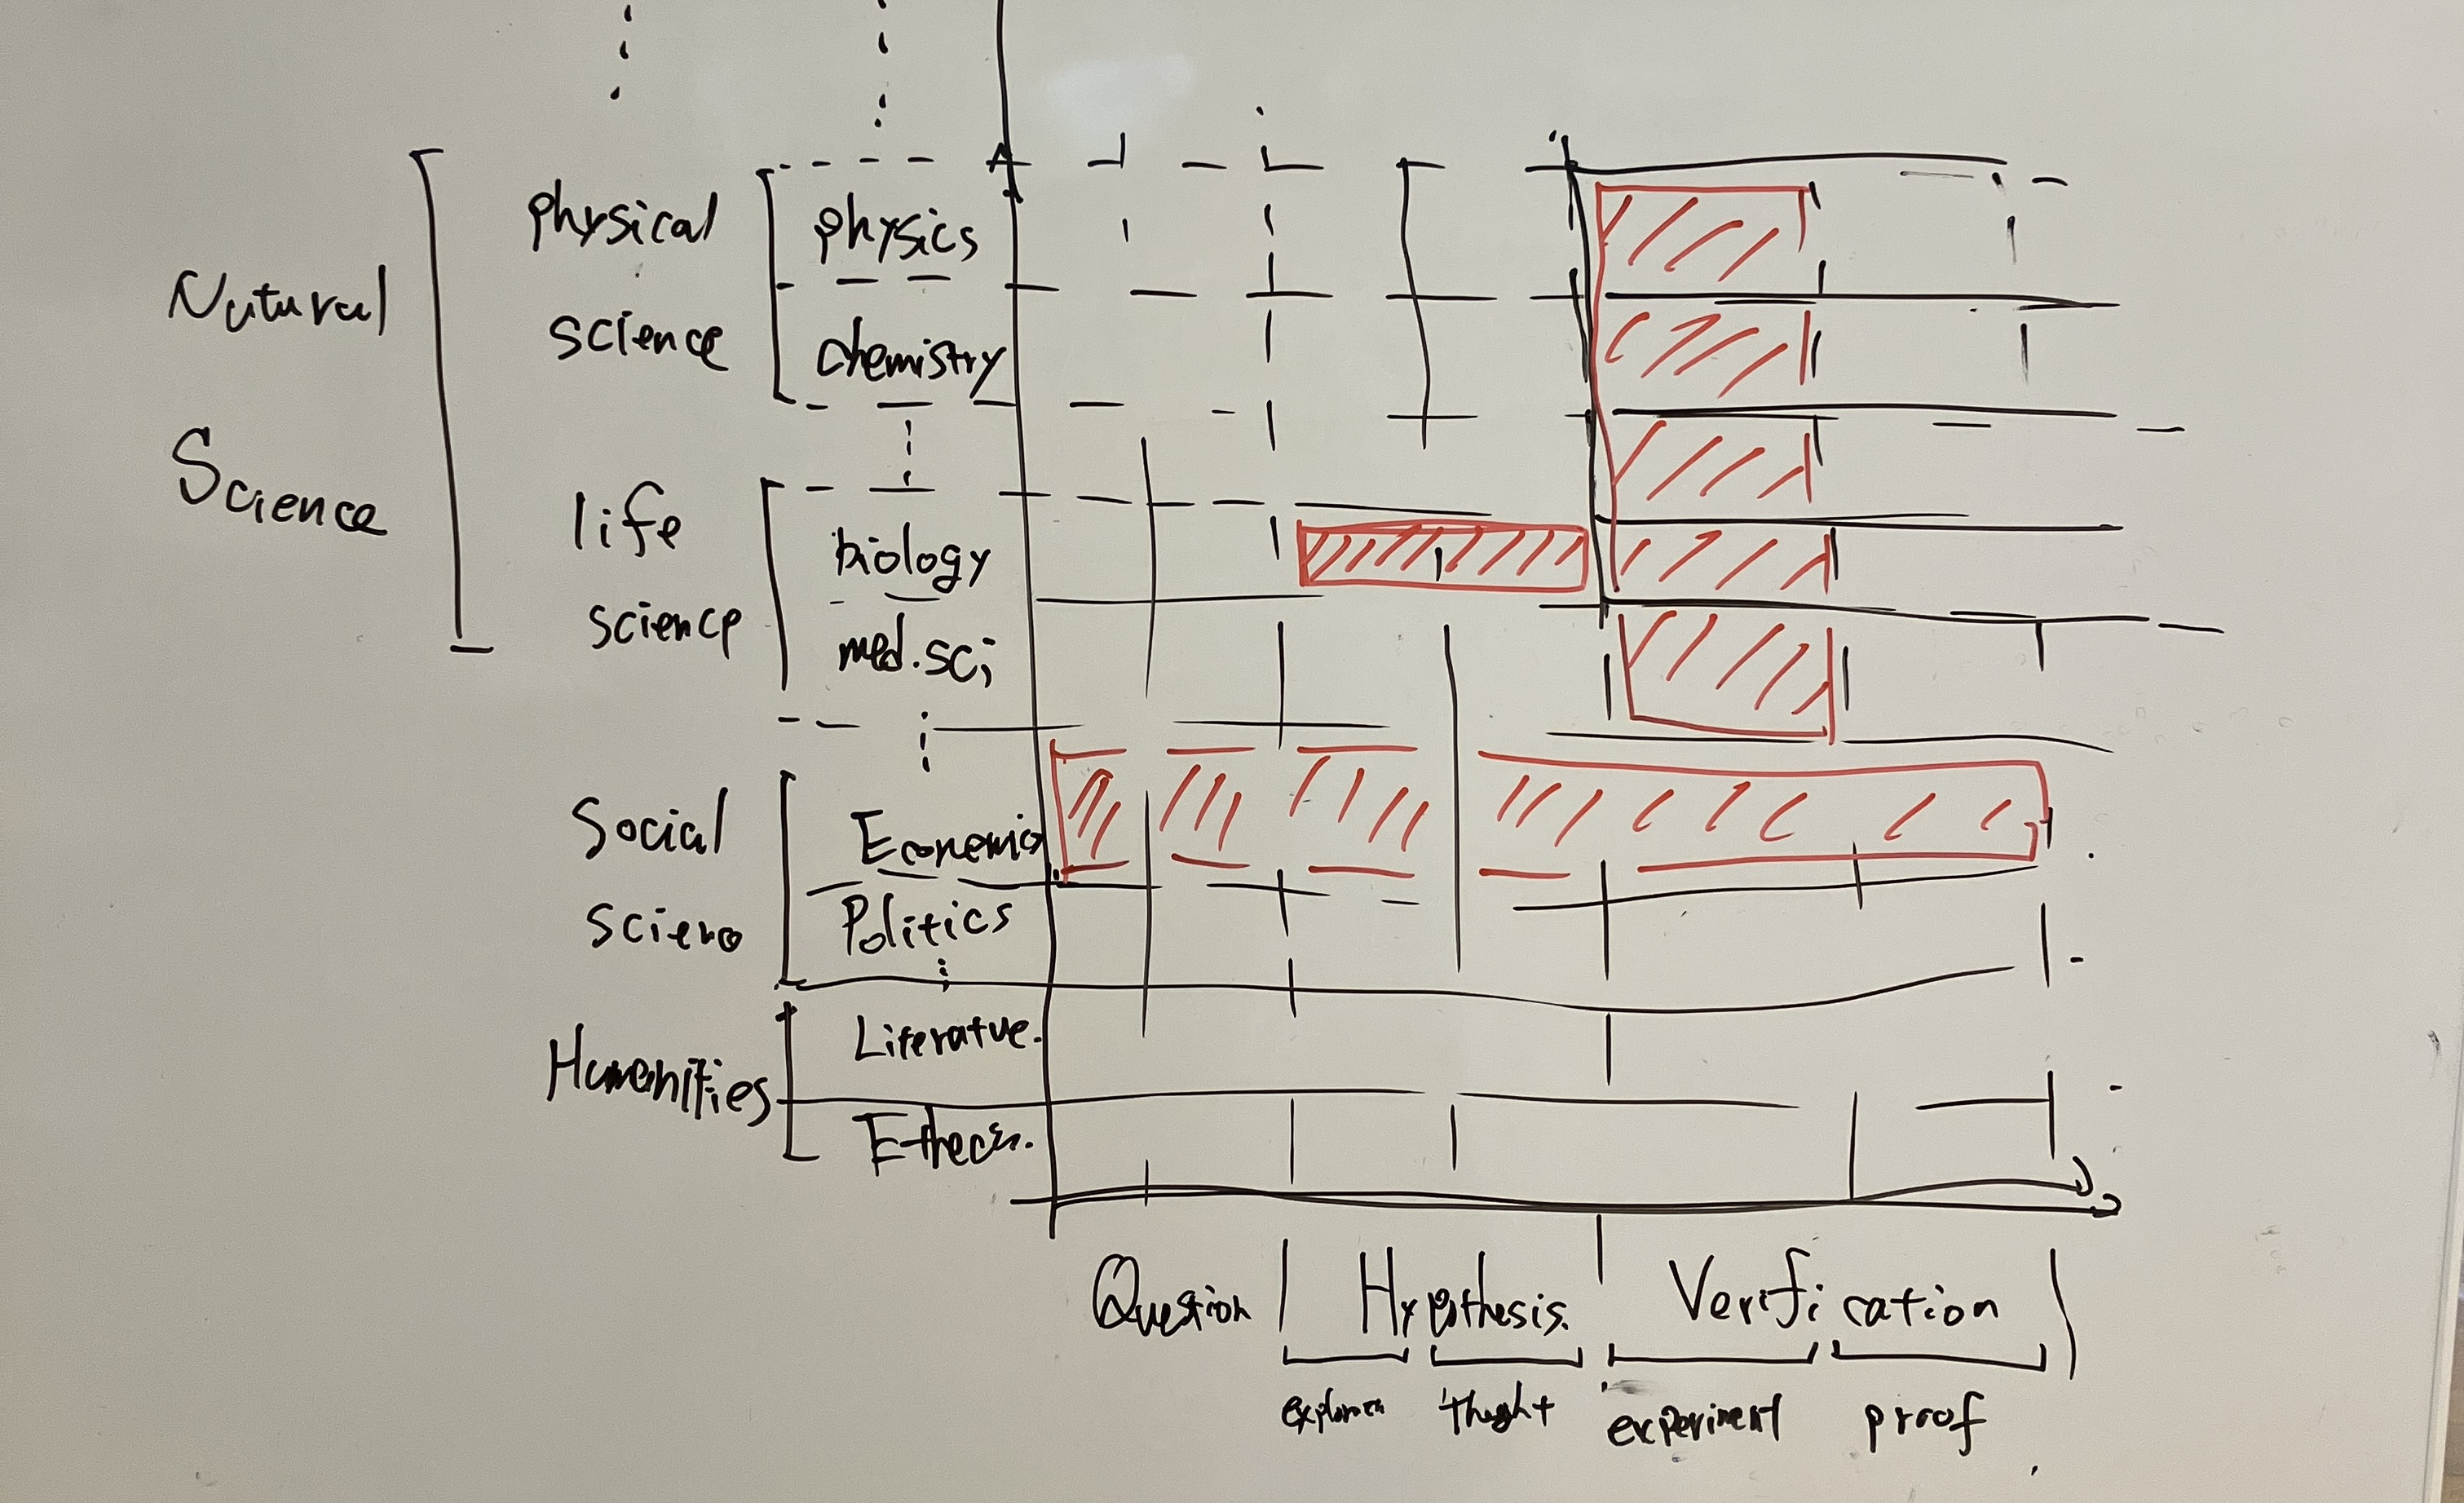
\includegraphics[width=\linewidth]{figs/generality_matrix.jpg}
%     \caption{Caption}
%     \label{fig:generality_matrix}
% \end{figure}

% Fig. \ref{fig:generality_matrix} conceptually illustrates the position of automation according to the axes of research field and research process. The vertical axis is the research field axis and the horizontal axis is the research process axis. Closer to the vertical axis corresponds to more specific research areas, and farther away from the vertical axis corresponds to a broader range of research areas. The horizontal axis corresponds to question construction, hypothesis generation, and hypothesis testing, from left to right, and is further divided within each category into more detailed e.g. empirical and non-empirical methods. Note that this is only a conceptual diagram and not an exact classification.

% As a example, the automation of protein structure prediction \cite{jumper2021highly} can be seen as the automation of a certain hypothesis generation task in a certain molecular biology study. The work of robot scientist \cite{king2004functional} can also be understood as an attempt to automate many of the steps in the study of identifying the function of genes in genetics, from hypothesis generation, to testing, to generating new hypotheses. (Explanation of the figure).

% Our goal of creating a versatile and autonomous artificial researcher is to automate everything on this two-dimensional surface. The area circled by the blue qualification in this figure corresponds to that. In other words, our goal is to realize an artificial intelligence that can autonomously execute any research or any process of research.



% \section{Others}

% Upon the completion of a study, the drafting of a manuscript, and its successful navigation of the peer-review process, the resulting findings are deemed to possess a degree of credibility as knowledge. Naturally, it would be hasty to assert that this alone births ``correct'' knowledge, as research demands iterative verification to confirm its validity. We convey such knowledge to others through various means, one of which is the presentation of research findings. To effectively communicate these outcomes, we create slides that elucidate our work. Studies also exist that strive to automate this aspect of the dissemination process \cite{sefid2019automatic}.

\section{Conclusion}
In this chapter, we briefly introduced initiatives related to the automation of research. Various efforts related to the automation of research are being carried out under different names in different communities. If information exchange between these communities becomes more active, the movement towards realizing AI capable of conducting research will likely accelerate.

Next, we briefly explained how these initiatives can be associated with the processes of question formulation, hypothesis generation, and hypothesis verification.

Lastly, we characterized these efforts from the perspectives of autonomy and generality. We point out that there have been significant development to achieve high autonomy or generality. However, we notice that there are still significant challenges to realizing complete autonomy or generality. In particular, there are still many challenges to realizing an AI capable of conducting research that achieves both generality and autonomy at a high level.